%$$$$$$$$$$$$$$$$$$$$$$$$$$$$$$$$$$$$$$$$$$$$$$$$$$$$$$$$$$$$$$$$$$$$$$$$$$$$$$$$
% Paragraph 3: Scalable Data Structure and Lock에 대한 연구
%$$$$$$$$$$$$$$$$$$$$$$$$$$$$$$$$$$$$$$$$$$$$$$$$$$$$$$$$$$$$$$$$$$$$$$$$$$$$$$$$
\newpage
\section{확장성 있는 락 연구}
\label{sec:lockrelated}

%$$$$$$$$$$$$$$$$$$$$$$$$$$$$$$$$$$$$$$$$$$$$$$$$$$$$$$$$$$$$$$$$$$$$$$$$$$$$$$$$
%Paragraph : 기본적인 락에 대한 이야기와 확장성 있는 락의 필요성 
%$$$$$$$$$$$$$$$$$$$$$$$$$$$$$$$$$$$$$$$$$$$$$$$$$$$$$$$$$$$$$$$$$$$$$$$$$$$$$$$$
락은 기본적으로 여러 스레드들을 안전하고 올바르게 동작하도록 만들어주는 방법이다. 
이처럼 여러 스레드를 안전하게 동작시켜주기 위해, 락은 하드웨어 동기화 명령들(CAS(Compare-And-Swap),
fetch-and-add, SWAP 등)을 이용하여 구현된다.
기본적으로 락의 구현은 코어들과 RAM간에는 공유하는 버스가 있고, 이러한 버스를 이용하여 원자적으로 처리하기 위해 
하드웨어 동기화 명령을 사용하여 구현한다. 
예를 들어 x86 시스템 같은 경우 xchg 명령어를 통해 락을 쉽게 구현할 수 있다.
하지만 실제 시스템은 보다 더 복잡한 구조를점 가지게 되는데, 
복잡한 이유는 중간에 캐시 메모리와 일관성을 유지하기 위한 
캐시 일관성 프로토콜과 매니코어 NUMA 구조에 최적화 되도록 구현해야 하기 때문이다.

%$$$$$$$$$$$$$$$$$$$$$$$$$$$$$$$$$$$$$$$$$$$$$$$$$$$$$$$$$$$$$$$$$$$$$$$$$$$$$$$$
%Paragraph : 리눅스 락 구현에 대한 이야기
%$$$$$$$$$$$$$$$$$$$$$$$$$$$$$$$$$$$$$$$$$$$$$$$$$$$$$$$$$$$$$$$$$$$$$$$$$$$$$$$$

이처럼 락의 primitive들은 기본적으로 두 종류로 구현되어 있는데, 


Non-blocking synchronization은 장점은 여러 스레드들이 락 기반으로 자원을 관리함에 따라
 발생하는 문제를 해결할 수 있다. 
가장 큰 장점은 스레드 또는 프로세스가 락 때문에 기다리는 시간을 제거할 수 있다.
이 것은 락을 얻기 위해 기다리는 시간을 최소화 할 뿐만 아니라 무한 루프 때문에 무한정 기다리는 
데드락 같은 상황까지 제거 할 수 있다. 
다음으로 모든 락은 락 자체의 오버헤드를 가지고 있는데 이것을 제거할 수 있다. 
예를 들어 코어 수가 증가 할 수록 락 자체를 얻기 위해 원자적 명령을 이용한느데 이것은 캐시 일관성 트래픽을 
발생한다. 
이와 같이 Non-blocking 방법은 이러한 락 자체가 가지고 있는 문제점인 데드락(deadlock), 라이브락(livelock), 
우선순위 역전현상(priority inversion)등을 제거 할 수 있다. 
이러한 Non-blocking synchronization 기법을 사용하는 lock-free 자료 구조들은 성능을 향상 시킬 수 있다. 
그 이유는 멀티코어 환경에서 공유되는 데이터를 접근하기 위해 직렬화 되는 부분이 매우 짧기 때문이다. 



%$$$$$$$$$$$$$$$$$$$$$$$$$$$$$$$$$$$$$$$$$$$$$$$$$$$$$$$$$$$$$$$$$$$$$$$$$$$$$$$$
%Paragraph : 락과 확장성에 대한 이야기
%$$$$$$$$$$$$$$$$$$$$$$$$$$$$$$$$$$$$$$$$$$$$$$$$$$$$$$$$$$$$$$$$$$$$$$$$$$$$$$$$

Non-blocking synchronization은 장점은 여러 스레드들이 락 기반으로 자원을 관리함에 따라
 발생하는 문제를 해결할 수 있다. 
가장 큰 장점은 스레드 또는 프로세스가 락 때문에 기다리는 시간을 제거할 수 있다.
이 것은 락을 얻기 위해 기다리는 시간을 최소화 할 뿐만 아니라 무한 루프 때문에 무한정 기다리는 
데드락 같은 상황까지 제거 할 수 있다. 
다음으로 모든 락은 락 자체의 오버헤드를 가지고 있는데 이것을 제거할 수 있다. 
예를 들어 코어 수가 증가 할 수록 락 자체를 얻기 위해 원자적 명령을 이용한느데 이것은 캐시 일관성 트래픽을 
발생한다. 
이와 같이 Non-blocking 방법은 이러한 락 자체가 가지고 있는 문제점인 데드락(deadlock), 라이브락(livelock), 
우선순위 역전현상(priority inversion)등을 제거 할 수 있다. 
이러한 Non-blocking synchronization 기법을 사용하는 lock-free 자료 구조들은 성능을 향상 시킬 수 있다. 
그 이유는 멀티코어 환경에서 공유되는 데이터를 접근하기 위해 직렬화 되는 부분이 매우 짧기 때문이다. 




%$$$$$$$$$$$$$$$$$$$$$$$$$$$$$$$$$$$$$$$$$$$$$$$$$$$$$$$$$$$$$$$$$$$$$$$$$$$$$$$$
%Paragraph :   cache coherence 이야기
%$$$$$$$$$$$$$$$$$$$$$$$$$$$$$$$$$$$$$$$$$$$$$$$$$$$$$$$$$$$$$$$$$$$$$$$$$$$$$$$$
Non-blocking synchronization은 장점은 여러 스레드들이 락 기반으로 자원을 관리함에 따라
 발생하는 문제를 해결할 수 있다. 
가장 큰 장점은 스레드 또는 프로세스가 락 때문에 기다리는 시간을 제거할 수 있다.
이 것은 락을 얻기 위해 기다리는 시간을 최소화 할 뿐만 아니라 무한 루프 때문에 무한정 기다리는 
데드락 같은 상황까지 제거 할 수 있다. 
다음으로 모든 락은 락 자체의 오버헤드를 가지고 있는데 이것을 제거할 수 있다. 
예를 들어 코어 수가 증가 할 수록 락 자체를 얻기 위해 원자적 명령을 이용한느데 이것은 캐시 일관성 트래픽을 
발생한다. 
이와 같이 Non-blocking 방법은 이러한 락 자체가 가지고 있는 문제점인 데드락(deadlock), 라이브락(livelock), 
우선순위 역전현상(priority inversion)등을 제거 할 수 있다. 
이러한 Non-blocking synchronization 기법을 사용하는 lock-free 자료 구조들은 성능을 향상 시킬 수 있다. 
그 이유는 멀티코어 환경에서 공유되는 데이터를 접근하기 위해 직렬화 되는 부분이 매우 짧기 때문이다. 

%how does cache coherence work?
 % many schemes, here's a simple one
  %each cache line: state, address, 64 bytes of data
  %states: Modified, Shared, Invalid [MSI]
  %cores exchange messages as they read and write

%messages (much simplified)
 % invalidate(addr): delete from your cache
%  find(addr): does any core have a copy?
 % all msgs are broadcast to all cores

%how do the cores coordinate with each other?
 % I + local read -> find, S
  %I + local write -> find, inval, M
  %S + local read -> S
  %S + local write -> inval, M
  %S + recv inval -> I
  %S + recv find  -> nothing, S
  %M + recv inval -> I
  %M + recv find  -> reply, S

%can read w/o bus traffic if already S
%can write w/o bus traffic if already M
 % "write-back"

%compatibility of states between 2 cores:

 %         core1
  %        M S I
   %     M - - +
%    core2   S - + +
 %       I + + +

%invariant: for each line, at most one core in M
%invariant: for each line, either one M or many S, never both

%Q: what patterns of use benefit from this coherence scheme?
 %  read-only data (every cache can have a copy)
  % data written multiple times by one core (M gives exclusive use, cheap
   % writes)

%other plans are possible
 % e.g. writes update copies rather than invalidating
  %but "write-invalidate" seems generally the best

%Real hardware uses much more clever schemes
  %mesh of links instead of bus; unicast instead of broadcast
   % "interconnect"
  %distributed directory to track which cores cache each line
   % unicast find to directory

%$$$$$$$$$$$$$$$$$$$$$$$$$$$$$$$$$$$$$$$$$$$$$$$$$$$$$$$$$$$$$$$$$$$$$$$$$$$$$$$$
%Paragraph :   atomic instructions 이야기
%$$$$$$$$$$$$$$$$$$$$$$$$$$$$$$$$$$$$$$$$$$$$$$$$$$$$$$$$$$$$$$$$$$$$$$$$$$$$$$$$

Non-blocking synchronization은 장점은 여러 스레드들이 락 기반으로 자원을 관리함에 따라
 발생하는 문제를 해결할 수 있다. 
가장 큰 장점은 스레드 또는 프로세스가 락 때문에 기다리는 시간을 제거할 수 있다.
이 것은 락을 얻기 위해 기다리는 시간을 최소화 할 뿐만 아니라 무한 루프 때문에 무한정 기다리는 
데드락 같은 상황까지 제거 할 수 있다. 
다음으로 모든 락은 락 자체의 오버헤드를 가지고 있는데 이것을 제거할 수 있다. 
예를 들어 코어 수가 증가 할 수록 락 자체를 얻기 위해 원자적 명령을 이용한느데 이것은 캐시 일관성 트래픽을 
발생한다. 
이와 같이 Non-blocking 방법은 이러한 락 자체가 가지고 있는 문제점인 데드락(deadlock), 라이브락(livelock), 
우선순위 역전현상(priority inversion)등을 제거 할 수 있다. 
이러한 Non-blocking synchronization 기법을 사용하는 lock-free 자료 구조들은 성능을 향상 시킬 수 있다. 
그 이유는 멀티코어 환경에서 공유되는 데이터를 접근하기 위해 직렬화 되는 부분이 매우 짧기 때문이다. 

%Q: why do we need locks if we have cache coherence?
 %  cache coherence ensures that cores read fresh data
  % locks avoid lost updates in read-modify-write cycles
   %  and prevent anyone from seeing partially updated data structures

%people build locks from h/w-supported atomic instructions
 % xv6 uses atomic exchange
  %other locks use test-and-set, atomic increment, &c
  %the __sync_... functions in the handout turn into atomic instructions

%how does the hardware implement atomic instructions?
%  get the line in M mode
%  defer coherence msgs
%  do all the steps (e.g. read old value, write new value)
%  resume processing msgs

%what is performance of locks?
 % assume N cores are waiting for the lock
  %how long does it take to hand off the lock?
   % from previous holder to next holder
  %bottleneck is usually the interconnect
   % so we'll measure cost in terms of # of msgs

%what performance could we hope for?
 % if N cores waiting,
  %get through them all in O(N) time
  %so each critical section and handoff takes O(1) time
   % i.e. does not increase with N


%$$$$$$$$$$$$$$$$$$$$$$$$$$$$$$$$$$$$$$$$$$$$$$$$$$$$$$$$$$$$$$$$$$$$$$$$$$$$$$$$
%Paragraph :   ts, ticket lock 이야기
%$$$$$$$$$$$$$$$$$$$$$$$$$$$$$$$$$$$$$$$$$$$$$$$$$$$$$$$$$$$$$$$$$$$$$$$$$$$$$$$$

Non-blocking synchronization은 장점은 여러 스레드들이 락 기반으로 자원을 관리함에 따라
 발생하는 문제를 해결할 수 있다. 
가장 큰 장점은 스레드 또는 프로세스가 락 때문에 기다리는 시간을 제거할 수 있다.
이 것은 락을 얻기 위해 기다리는 시간을 최소화 할 뿐만 아니라 무한 루프 때문에 무한정 기다리는 
데드락 같은 상황까지 제거 할 수 있다. 
다음으로 모든 락은 락 자체의 오버헤드를 가지고 있는데 이것을 제거할 수 있다. 
예를 들어 코어 수가 증가 할 수록 락 자체를 얻기 위해 원자적 명령을 이용한느데 이것은 캐시 일관성 트래픽을 
발생한다. 
이와 같이 Non-blocking 방법은 이러한 락 자체가 가지고 있는 문제점인 데드락(deadlock), 라이브락(livelock), 
우선순위 역전현상(priority inversion)등을 제거 할 수 있다. 
이러한 Non-blocking synchronization 기법을 사용하는 lock-free 자료 구조들은 성능을 향상 시킬 수 있다. 
그 이유는 멀티코어 환경에서 공유되는 데이터를 접근하기 위해 직렬화 되는 부분이 매우 짧기 때문이다. 


%test&set spinlock (xv6/jos)
 % waiting cores repeatedly execute e.g. atomic exchange
%  Q: is that a problem?
%  yes!
%    we don't care if waiting cores waste their own time
%    we do care if waiting cores slow lock holder!
%  time for critical section and release:
%    holder must wait in line for access to bus
 %   so holder's mem ops take O(N) time
  %  so handoff time takes O(N)

%Q: is O(N) handoff time a problem?
 %  yes! we wanted O(1) time
  % O(N) per handoff means all N cores takes O(N^2) time, not O(N)

%$$$$$$$$$$$$$$$$$$$$$$$$$$$$$$$$$$$$$$$$$$$$$$$$$$$$$$$$$$$$$$$$$$$$$$$$$$$$$$$$
%Paragraph 2:  ts, ticket lock 이야기 2
%$$$$$$$$$$$$$$$$$$$$$$$$$$$$$$$$$$$$$$$$$$$$$$$$$$$$$$$$$$$$$$$$$$$$$$$$$$$$$$$$
Non-blocking synchronization은 장점은 여러 스레드들이 락 기반으로 자원을 관리함에 따라
 발생하는 문제를 해결할 수 있다. 
가장 큰 장점은 스레드 또는 프로세스가 락 때문에 기다리는 시간을 제거할 수 있다.
이 것은 락을 얻기 위해 기다리는 시간을 최소화 할 뿐만 아니라 무한 루프 때문에 무한정 기다리는 
데드락 같은 상황까지 제거 할 수 있다. 
다음으로 모든 락은 락 자체의 오버헤드를 가지고 있는데 이것을 제거할 수 있다. 
예를 들어 코어 수가 증가 할 수록 락 자체를 얻기 위해 원자적 명령을 이용한느데 이것은 캐시 일관성 트래픽을 
발생한다. 
이와 같이 Non-blocking 방법은 이러한 락 자체가 가지고 있는 문제점인 데드락(deadlock), 라이브락(livelock), 
우선순위 역전현상(priority inversion)등을 제거 할 수 있다. 
이러한 Non-blocking synchronization 기법을 사용하는 lock-free 자료 구조들은 성능을 향상 시킬 수 있다. 
그 이유는 멀티코어 환경에서 공유되는 데이터를 접근하기 위해 직렬화 되는 부분이 매우 짧기 때문이다. 


%ticket locks (linux):
 % goal: read-only spin loop, rather than repeated atomic instruction
%  goal: fairness (turns out t-s locks aren't fair)
  %idea: assign numbers, wake up one at a time
%    avoid constant t-s atomic instructions by waiters
%  Q: why is it cheaper than t-s lock?
%  Q: why is it fair?
 % time analysis:
  %  what happens in acquire?
      %atomic increment -- O(1) broadcast msg
        %just once, not repeated
      %then read-only spin, no cost until next release
    %what happens after release?
      %invalidate msg for now_serving
      %N "find" msgs for each core to read now_serving
    %so handoff has cost O(N)
    %note: it was *reading* that was costly!
  %oops, just as bad O() cost as test-and-set

%jargon: test-and-set and ticket locks are "non-scalable" locks
  %== cost of single handoff increases with N

%is the cost of non-scalable locks a serious problem?
 % after all, programs do lots of other things than locking
  %maybe locking cost is tiny compared to other stuff
  


이러한 락에 대한 연구는 확장성 있는 락들은 큐 기반의
락~\cite{MellorCrummey1991MCS}~\cite{Magnusson1994QLC}, ~\cite{Wang2016BeMyGuest},
~\cite{Scott2013SS}
~\cite{Bueso2014MCS}~\cite{Bueso2015STP}과 계층적
락~\cite{Radovic2003HBL}~\cite{Chabbi2016CLL}~\cite{Luchangco2006HCQ}
~\cite{Chabbi2015HPL} 그리고 위임하는 방법(delegation
techniques)~\cite{Hendler2010FC}~\cite{Fatourou2012RCS}~\cite{Delegation2014}들이
연구되고 있다. 

\subsection{큐 기반의 락(Queued Lock)}


\subsubsection{MCS}

%$$$$$$$$$$$$$$$$$$$$$$$$$$$$$$$$$$$$$$$$$$$$$$$$$$$$$$$$$$$$$$$$$$$$$$$$$$$$$$$$
%Paragraph :   MCS 이야기
%$$$$$$$$$$$$$$$$$$$$$$$$$$$$$$$$$$$$$$$$$$$$$$$$$$$$$$$$$$$$$$$$$$$$$$$$$$$$$$$$

Non-blocking synchronization은 장점은 여러 스레드들이 락 기반으로 자원을 관리함에 따라
 발생하는 문제를 해결할 수 있다. 
가장 큰 장점은 스레드 또는 프로세스가 락 때문에 기다리는 시간을 제거할 수 있다.
이 것은 락을 얻기 위해 기다리는 시간을 최소화 할 뿐만 아니라 무한 루프 때문에 무한정 기다리는 
데드락 같은 상황까지 제거 할 수 있다. 
다음으로 모든 락은 락 자체의 오버헤드를 가지고 있는데 이것을 제거할 수 있다. 
예를 들어 코어 수가 증가 할 수록 락 자체를 얻기 위해 원자적 명령을 이용한느데 이것은 캐시 일관성 트래픽을 
발생한다. 
이와 같이 Non-blocking 방법은 이러한 락 자체가 가지고 있는 문제점인 데드락(deadlock), 라이브락(livelock), 
우선순위 역전현상(priority inversion)등을 제거 할 수 있다. 
이러한 Non-blocking synchronization 기법을 사용하는 lock-free 자료 구조들은 성능을 향상 시킬 수 있다. 
그 이유는 멀티코어 환경에서 공유되는 데이터를 접근하기 위해 직렬화 되는 부분이 매우 짧기 때문이다. 


%see paper's Figure 2
 % let's consider Figure 2(c), PFIND -- parallel find
%  x-axis is # of cores, y-axis is finds completed per second (total throughput)
 % why does it go up?
%  why does it level off?
  %why does it go *down*?
  %what governs how far up it goes -- i.e. the max throughput?
  %why does it go down so steeply?

%reason for suddenness of collapse
 % serial section takes 7% on one core (Figure 3, last column)
  %so w/ 14 cores you'd expect just one or two in crit section
  %so it seems odd that collapse happens so soon
  %BUT:
   % once P(two cores waiting for lock) is substantial,
    %critical section + handoff starts taking longer
    %so starts to be more than 7%
    %so more cores end up waiting
    %so N grows, and thus handoff time, and thus N...

%some perspective
 % acquire(l)
%  x++
 % release(l)
  %surely a critical section this short cannot affect overall performance?
  %takes a few dozen cycles if same core last held the lock (still in M)
   % everything operates out of the cache, very fast
  %a hundred cycles if lock is not held and some other core previously held it
  %10,000 if contended by dozens of cores
  %many kernel operations only take a few 100 cycles total
   % so a contended lock may increase cost not by a few percent
    %but by 100x!

%how to make locks scale well?
 % we want just O(1) msgs during a release
%  how to cause only one core to read/write lock after a release?
 % how to wake up just one core at a time?

%Idea:
 % what if each core spins on a *different* cache line?
  %acquire cost?
   % atomic increment, then read-only spin
  %release cost?
   % invalidate next holder's slots[]
    %only they have to re-load
    %no other cores involved
  %so O(1) per release -- victory!
   % problem: high space cost
    %N slots per lock
    %often much more than size of protected object
    %(this solution is due to Anderson et al.)

%MCS
 % [diagram, code in handout]
  %goal: as scalable as anderson, but less space used
  %idea: linked list of waiters per lock
  %idea: one list element per thread, since a thread can wait on only one lock
   % so total space is O(locks + threads), not O(locks*threads)
  %acquire() pushes caller's element at end of list
   % caller then spins on a variable in its own element
  %release() wakes up next element, pops its own element
  %change in API (need to pass qnode to acquire and release to qnode allocation)

%performance of scalable locks?
%  figure 10 shows ticket, MCS, and optimized backoff
 % # cores on x-axis, total throughput on y-axis
  %benchmark acquires and releases, critical section dirties four cache lines
  %Q: why doesn't throughput go up as you add more cores?
  %ticket is best on two cores -- just one atomic instruction
  %ticket scales badly: cost goes up with more cores
  %MCS scales well: cost stays the same with more cores

%Figure 11 shows uncontended cost
 % very fast if no contention!
  %ticket:
   % acquire uses a single atomic instruction, so 10x more expensive than
    % release some what more expensive if so another core had it last

%Do scalable locks make the kernel scale better?
 % No. Scalability is limited by length of critical section
  %  Scalable locks avoid collapse
  %To fix scalability, need to redesign kernel subsystem
   % An example of redesign in next lecture


%$$$$$$$$$$$$$$$$$$$$$$$$$$$$$$$$$$$$$$$$$$$$$$$$$$$$$$$$$$$$$$$$$$$$$$$$$$$$$$$$
%Paragraph 2: scalable locks의 성능에 대한 이야
%$$$$$$$$$$$$$$$$$$$$$$$$$$$$$$$$$$$$$$$$$$$$$$$$$$$$$$$$$$$$$$$$$$$$$$$$$$$$$$$$
Non-blocking synchronization은 장점은 여러 스레드들이 락 기반으로 자원을 관리함에 따라
 발생하는 문제를 해결할 수 있다. 
가장 큰 장점은 스레드 또는 프로세스가 락 때문에 기다리는 시간을 제거할 수 있다.
이 것은 락을 얻기 위해 기다리는 시간을 최소화 할 뿐만 아니라 무한 루프 때문에 무한정 기다리는 
데드락 같은 상황까지 제거 할 수 있다. 
다음으로 모든 락은 락 자체의 오버헤드를 가지고 있는데 이것을 제거할 수 있다. 
예를 들어 코어 수가 증가 할 수록 락 자체를 얻기 위해 원자적 명령을 이용한느데 이것은 캐시 일관성 트래픽을 
발생한다. 
이와 같이 Non-blocking 방법은 이러한 락 자체가 가지고 있는 문제점인 데드락(deadlock), 라이브락(livelock), 
우선순위 역전현상(priority inversion)등을 제거 할 수 있다. 
이러한 Non-blocking synchronization 기법을 사용하는 lock-free 자료 구조들은 성능을 향상 시킬 수 있다. 
그 이유는 멀티코어 환경에서 공유되는 데이터를 접근하기 위해 직렬화 되는 부분이 매우 짧기 때문이다. 


%Notes on Linux and MCS locks (thanks to Srivatsa)

%The Linux kernel has scalable (or non-collapsing) locks and is using it.  One
% of the earliest efforts to fix the performance of ticket-based spinlocks dates
% back to 2013[1], and appears to have used the paper we read today as
% motivation. (But that particular patchset never actually made it to the
% mainline kernel). MCS locks found their way into the mutex-lock implementation
% at around the same time[2].
 
%Replacing ticket-spinlocks with scalable locks, however, turned out to be a
% much harder problem because locking schemes such as MCS would bloat the size of each
%spin-lock, which was undesirable due to additional constraints on the spin-lock
%size in the Linux kernel.

%A few years later, the Linux developers came up with “qspinlocks” (which
% use MCS underneath, with special tricks to avoid bloating the size of the spin-lock) to
%replace ticket-spinlocks, which is now the default spin-lock implementation in
%the Linux kernel since 2015[3][4].  You may also find this article[5] (written
%by one of the contributors to the Linux locking subsystem) quite interesting in
%this context.

%The old and unused ticket-spinlock implementation was deleted from the codebase
%in 2016[6].
 
%[1]. Fixing ticket-spinlocks:
 %     https://lwn.net/Articles/531254/
  %    https://lwn.net/Articles/530458/
 
%[2]. MCS locks used in the mutex-lock implementation:
 %    
      % http://git.kernel.org/cgit/linux/kernel/git/torvalds/linux.git/commit/?id=2bd2c92cf07cc4a
 
%[3]. MCS locks and qspinlocks:
 %     https://lwn.net/Articles/590243/
 
%[4]. qspinlock (using MCS underneath) as the default spin-lock implementation:
 %    
      % http://git.kernel.org/cgit/linux/kernel/git/torvalds/linux.git/commit/?id=a33fda35e3a765
 
%[5]. Article providing context and motivation for various locking schemes:
 %     http://queue.acm.org/detail.cfm?id=2698990
 
%[6]. Removal of unused ticket-spinlock code from the Linux kernel:
 %    
      % http://git.kernel.org/cgit/linux/kernel/git/torvalds/linux.git/commit/?id=cfd8983f03c7b2
      

\subsection{계층적 락}

~\cite{Dice2015LCG}

%$$$$$$$$$$$$$$$$$$$$$$$$$$$$$$$$$$$$$$$$$$$$$$$$$$$$$$$$$$$$$$$$$$$$$$$$$$$$$$$$
%Paragraph 2: 계층적 락
%$$$$$$$$$$$$$$$$$$$$$$$$$$$$$$$$$$$$$$$$$$$$$$$$$$$$$$$$$$$$$$$$$$$$$$$$$$$$$$$$
Non-blocking synchronization은 장점은 여러 스레드들이 락 기반으로 자원을 관리함에 따라
 발생하는 문제를 해결할 수 있다. 
가장 큰 장점은 스레드 또는 프로세스가 락 때문에 기다리는 시간을 제거할 수 있다.
이 것은 락을 얻기 위해 기다리는 시간을 최소화 할 뿐만 아니라 무한 루프 때문에 무한정 기다리는 
데드락 같은 상황까지 제거 할 수 있다. 
다음으로 모든 락은 락 자체의 오버헤드를 가지고 있는데 이것을 제거할 수 있다. 
예를 들어 코어 수가 증가 할 수록 락 자체를 얻기 위해 원자적 명령을 이용한느데 이것은 캐시 일관성 트래픽을 
발생한다. 
이와 같이 Non-blocking 방법은 이러한 락 자체가 가지고 있는 문제점인 데드락(deadlock), 라이브락(livelock), 
우선순위 역전현상(priority inversion)등을 제거 할 수 있다. 
이러한 Non-blocking synchronization 기법을 사용하는 lock-free 자료 구조들은 성능을 향상 시킬 수 있다. 
그 이유는 멀티코어 환경에서 공유되는 데이터를 접근하기 위해 직렬화 되는 부분이 매우 짧기 때문이다. 


\subsection{Delegation techniques}

\subsubsection{Flat Combining}

%$$$$$$$$$$$$$$$$$$$$$$$$$$$$$$$$$$$$$$$$$$$$$$$$$$$$$$$$$$$$$$$$$$$$$$$$$$$$$$$$
%Paragraph :   Flat Combining 이야기
%$$$$$$$$$$$$$$$$$$$$$$$$$$$$$$$$$$$$$$$$$$$$$$$$$$$$$$$$$$$$$$$$$$$$$$$$$$$$$$$$

Non-blocking synchronization은 장점은 여러 스레드들이 락 기반으로 자원을 관리함에 따라
 발생하는 문제를 해결할 수 있다. 
가장 큰 장점은 스레드 또는 프로세스가 락 때문에 기다리는 시간을 제거할 수 있다.
이 것은 락을 얻기 위해 기다리는 시간을 최소화 할 뿐만 아니라 무한 루프 때문에 무한정 기다리는 
데드락 같은 상황까지 제거 할 수 있다. 
다음으로 모든 락은 락 자체의 오버헤드를 가지고 있는데 이것을 제거할 수 있다. 
예를 들어 코어 수가 증가 할 수록 락 자체를 얻기 위해 원자적 명령을 이용한느데 이것은 캐시 일관성 트래픽을 
발생한다. 
이와 같이 Non-blocking 방법은 이러한 락 자체가 가지고 있는 문제점인 데드락(deadlock), 라이브락(livelock), 
우선순위 역전현상(priority inversion)등을 제거 할 수 있다. 
이러한 Non-blocking synchronization 기법을 사용하는 lock-free 자료 구조들은 성능을 향상 시킬 수 있다. 
그 이유는 멀티코어 환경에서 공유되는 데이터를 접근하기 위해 직렬화 되는 부분이 매우 짧기 때문이다. 

\begin{figure}[h!]
    \centering
    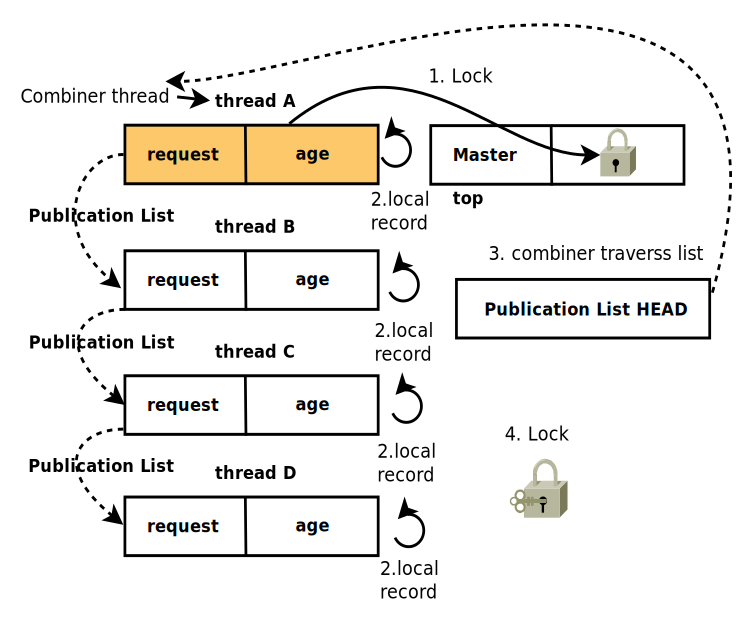
\includegraphics[width=1\textwidth]{fig/FC/FC}
    \caption{Flat combining 방법}
  \label{fig:FC}
\end{figure}

%Flat combining in shared memory.
%To access the shared stack, each thread adds its request
%to the publication list (1). Thread 4 acquires the stack’s lock and becomes the
% combiner (2), while the remaining threads spin waiting for their request to be satisfied. The combiner walks the publication list
%from the head, matching up Thread 3’s push with Thread 2’s pop on its own
% private stack (3). The two remaining pushes are added to the top of the
% shared stack (4). Finally, the top is updated, and Thread 4
%releases the lock and continues its normal executio

%$$$$$$$$$$$$$$$$$$$$$$$$$$$$$$$$$$$$$$$$$$$$$$$$$$$$$$$$$$$$$$$$$$$$$$$$$$$$$$$$
%Paragraph :   Flat Combining 알고리즘
%$$$$$$$$$$$$$$$$$$$$$$$$$$$$$$$$$$$$$$$$$$$$$$$$$$$$$$$$$$$$$$$$$$$$$$$$$$$$$$$$

Non-blocking synchronization은 장점은 여러 스레드들이 락 기반으로 자원을 관리함에 따라
 발생하는 문제를 해결할 수 있다. 
가장 큰 장점은 스레드 또는 프로세스가 락 때문에 기다리는 시간을 제거할 수 있다.
이 것은 락을 얻기 위해 기다리는 시간을 최소화 할 뿐만 아니라 무한 루프 때문에 무한정 기다리는 
데드락 같은 상황까지 제거 할 수 있다. 
다음으로 모든 락은 락 자체의 오버헤드를 가지고 있는데 이것을 제거할 수 있다. 
예를 들어 코어 수가 증가 할 수록 락 자체를 얻기 위해 원자적 명령을 이용한느데 이것은 캐시 일관성 트래픽을 
발생한다. 
이와 같이 Non-blocking 방법은 이러한 락 자체가 가지고 있는 문제점인 데드락(deadlock), 라이브락(livelock), 
우선순위 역전현상(priority inversion)등을 제거 할 수 있다. 
이러한 Non-blocking synchronization 기법을 사용하는 lock-free 자료 구조들은 성능을 향상 시킬 수 있다. 
그 이유는 멀티코어 환경에서 공유되는 데이터를 접근하기 위해 직렬화 되는 부분이 매우 짧기 때문이다. 




\subsubsection{OpLog}

OpLog는 RCU와 반대로 업데이트 비율이 높은 업데이트 헤비(Update heavy)한 자료구조를 위해 만든 
동기화 기법 중 하나이다.

%$$$$$$$$$$$$$$$$$$$$$$$$$$$$$$$$$$$$$$$$$$$$$$$$$$$$$$$$$$$$$$$$$$$$$$$$$$$$$$$$
%Paragraph 2: OpLog 이야기
%$$$$$$$$$$$$$$$$$$$$$$$$$$$$$$$$$$$$$$$$$$$$$$$$$$$$$$$$$$$$$$$$$$$$$$$$$$$$$$$$
Non-blocking synchronization은 장점은 여러 스레드들이 락 기반으로 자원을 관리함에 따라
 발생하는 문제를 해결할 수 있다. 
가장 큰 장점은 스레드 또는 프로세스가 락 때문에 기다리는 시간을 제거할 수 있다.
이 것은 락을 얻기 위해 기다리는 시간을 최소화 할 뿐만 아니라 무한 루프 때문에 무한정 기다리는 
데드락 같은 상황까지 제거 할 수 있다. 
다음으로 모든 락은 락 자체의 오버헤드를 가지고 있는데 이것을 제거할 수 있다. 
예를 들어 코어 수가 증가 할 수록 락 자체를 얻기 위해 원자적 명령을 이용한느데 이것은 캐시 일관성 트래픽을 
발생한다. 
이와 같이 Non-blocking 방법은 이러한 락 자체가 가지고 있는 문제점인 데드락(deadlock), 라이브락(livelock), 
우선순위 역전현상(priority inversion)등을 제거 할 수 있다. 
이러한 Non-blocking synchronization 기법을 사용하는 lock-free 자료 구조들은 성능을 향상 시킬 수 있다. 
그 이유는 멀티코어 환경에서 공유되는 데이터를 접근하기 위해 직렬화 되는 부분이 매우 짧기 때문이다. 


\begin{figure}[h]
    \centering
    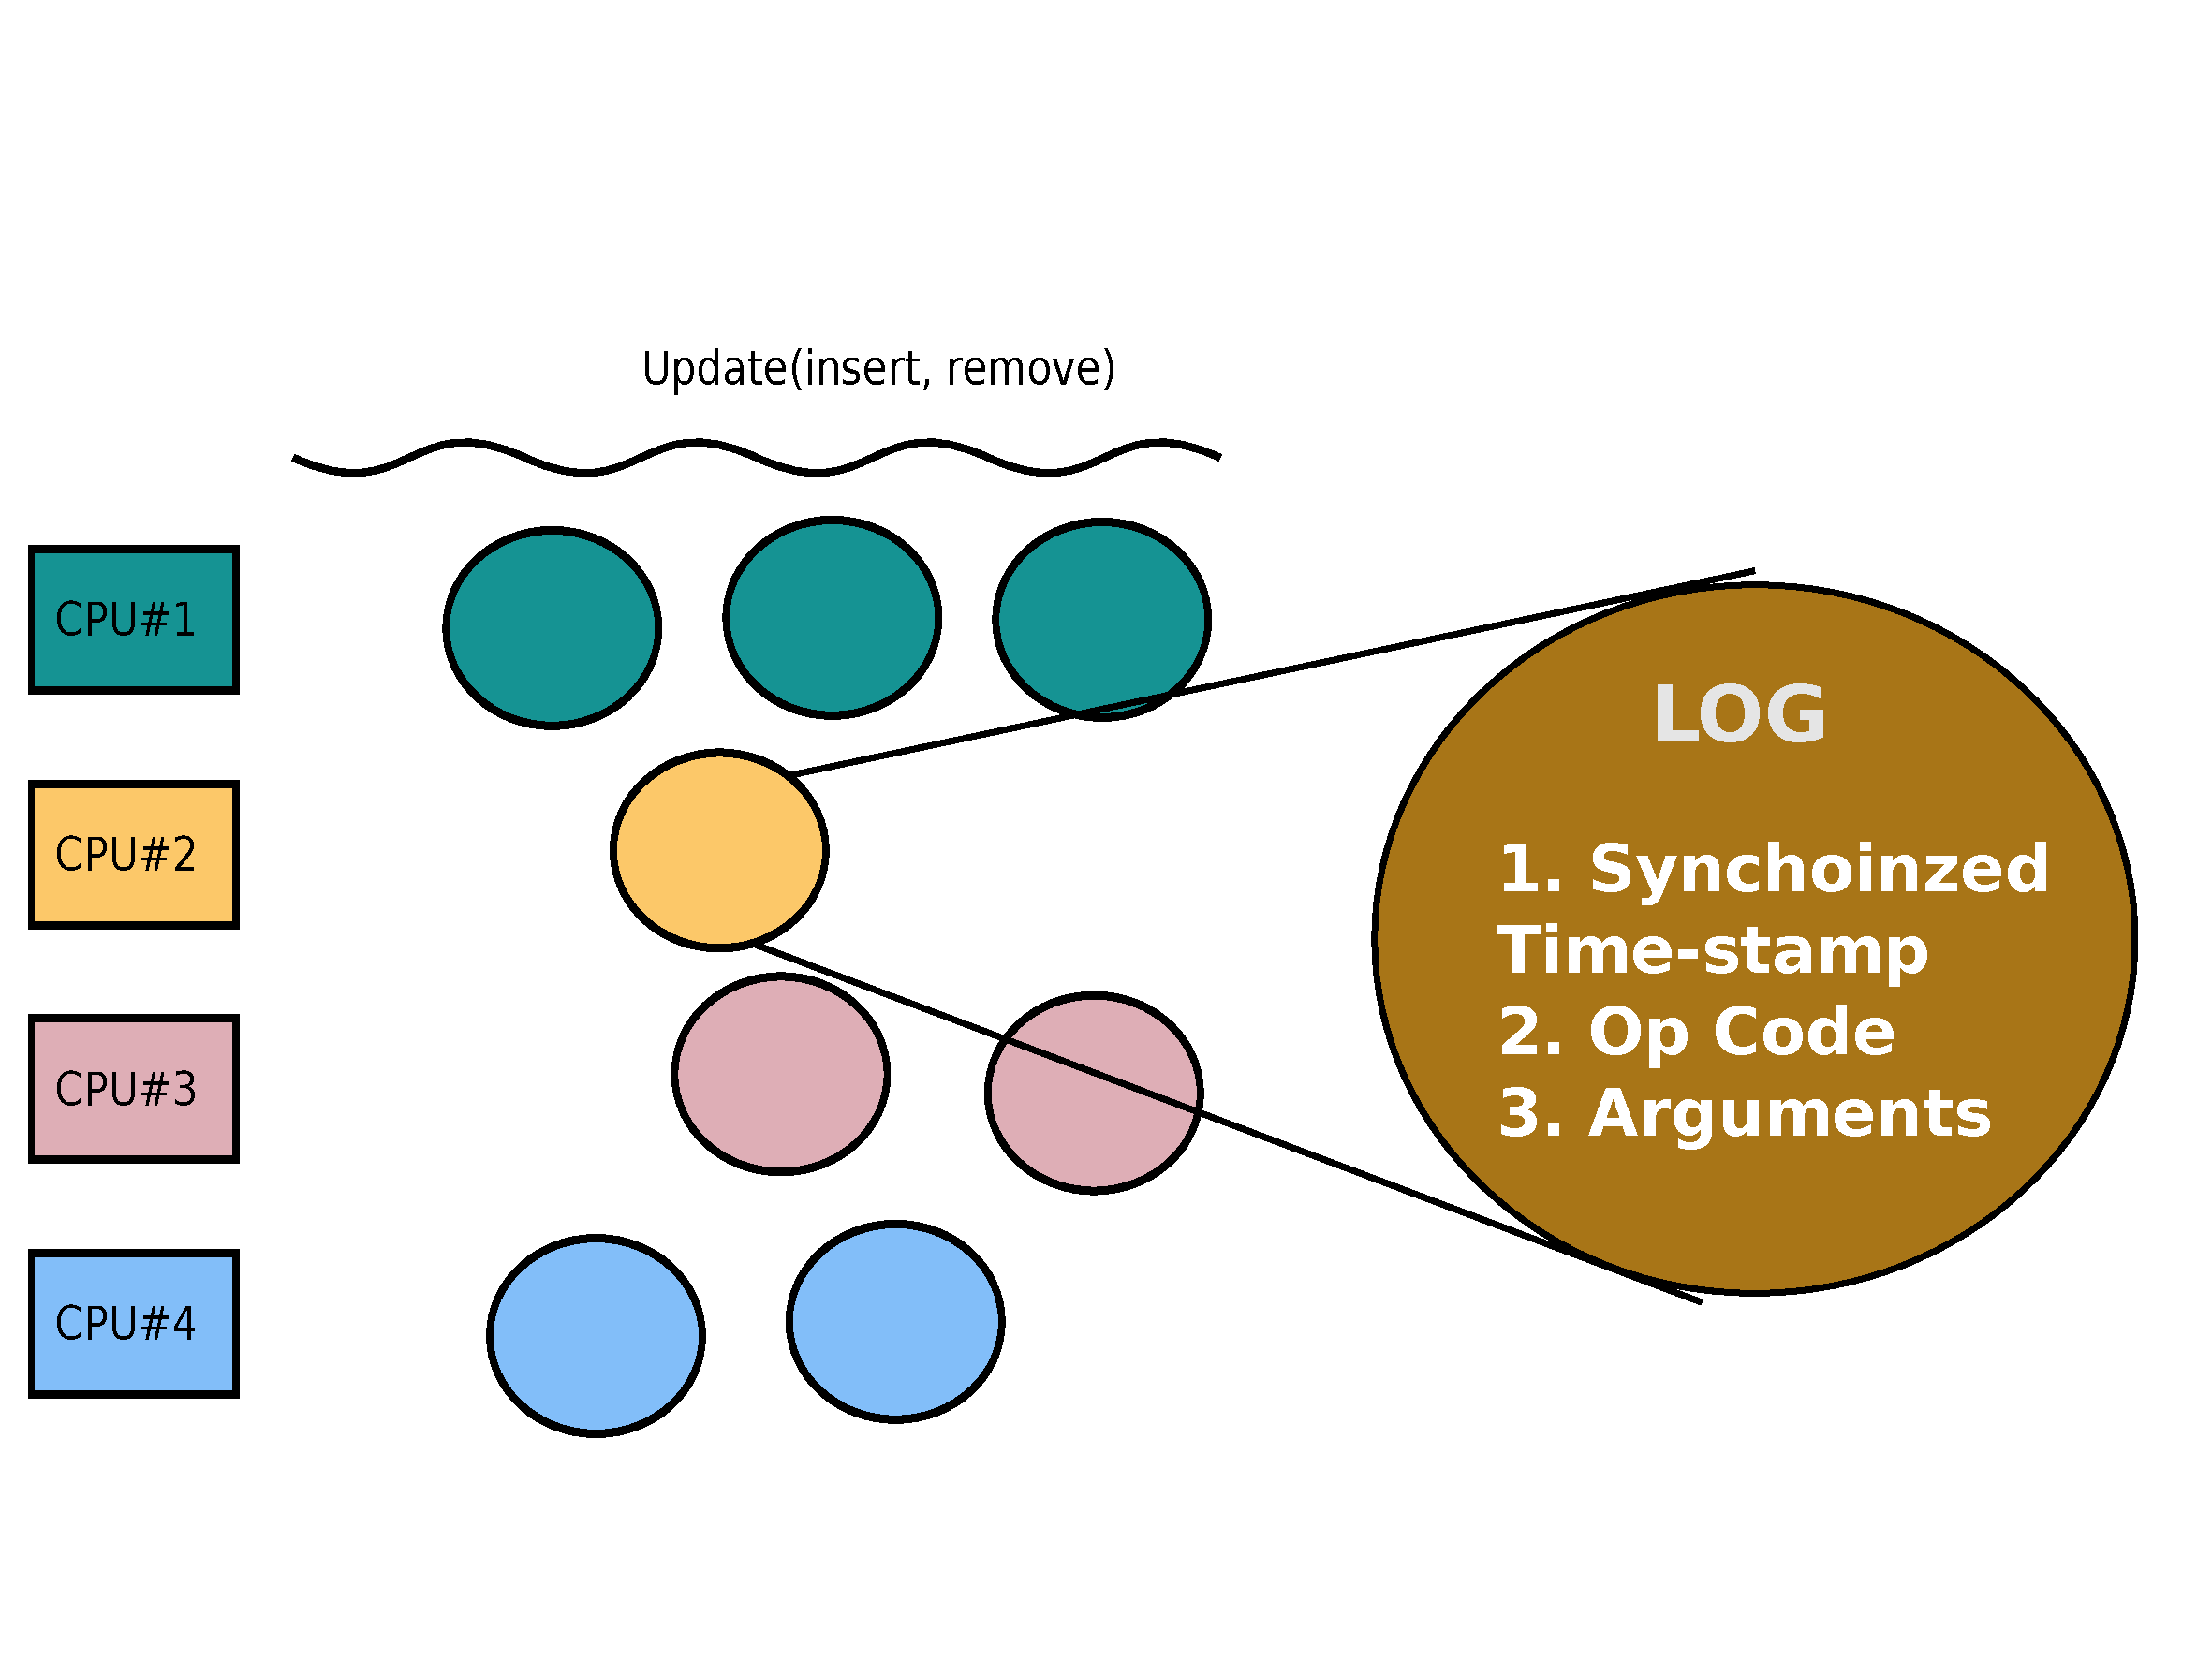
\includegraphics[width=0.8\textwidth]{fig/oplog_log}
    \caption{OpLog의 업데이트 방법}
  \label{fig:oplog}
\end{figure}


%$$$$$$$$$$$$$$$$$$$$$$$$$$$$$$$$$$$$$$$$$$$$$$$$$$$$$$$$$$$$$$$$$$$$$$$$$$$$$$$$
%Paragraph 2: OpLog의 작전
%$$$$$$$$$$$$$$$$$$$$$$$$$$$$$$$$$$$$$$$$$$$$$$$$$$$$$$$$$$$$$$$$$$$$$$$$$$$$$$$$
Non-blocking synchronization은 장점은 여러 스레드들이 락 기반으로 자원을 관리함에 따라
 발생하는 문제를 해결할 수 있다. 
가장 큰 장점은 스레드 또는 프로세스가 락 때문에 기다리는 시간을 제거할 수 있다.
이 것은 락을 얻기 위해 기다리는 시간을 최소화 할 뿐만 아니라 무한 루프 때문에 무한정 기다리는 
데드락 같은 상황까지 제거 할 수 있다. 
다음으로 모든 락은 락 자체의 오버헤드를 가지고 있는데 이것을 제거할 수 있다. 
예를 들어 코어 수가 증가 할 수록 락 자체를 얻기 위해 원자적 명령을 이용한느데 이것은 캐시 일관성 트래픽을 
발생한다. 
이와 같이 Non-blocking 방법은 이러한 락 자체가 가지고 있는 문제점인 데드락(deadlock), 라이브락(livelock), 
우선순위 역전현상(priority inversion)등을 제거 할 수 있다. 
이러한 Non-blocking synchronization 기법을 사용하는 lock-free 자료 구조들은 성능을 향상 시킬 수 있다. 
그 이유는 멀티코어 환경에서 공유되는 데이터를 접근하기 위해 직렬화 되는 부분이 매우 짧기 때문이다. 

%$$$$$$$$$$$$$$$$$$$$$$$$$$$$$$$$$$$$$$$$$$$$$$$$$$$$$$$$$$$$$$$$$$$$$$$$$$$$$$$$
%Paragraph 2: OpLog의 문제
%$$$$$$$$$$$$$$$$$$$$$$$$$$$$$$$$$$$$$$$$$$$$$$$$$$$$$$$$$$$$$$$$$$$$$$$$$$$$$$$$
Non-blocking synchronization은 장점은 여러 스레드들이 락 기반으로 자원을 관리함에 따라
 발생하는 문제를 해결할 수 있다. 
가장 큰 장점은 스레드 또는 프로세스가 락 때문에 기다리는 시간을 제거할 수 있다.
이 것은 락을 얻기 위해 기다리는 시간을 최소화 할 뿐만 아니라 무한 루프 때문에 무한정 기다리는 
데드락 같은 상황까지 제거 할 수 있다. 
다음으로 모든 락은 락 자체의 오버헤드를 가지고 있는데 이것을 제거할 수 있다. 
예를 들어 코어 수가 증가 할 수록 락 자체를 얻기 위기해 원자적 명령을 이용한느데 이것은 캐시 일관성 트래픽을 
발생한다. 
이와 같이 Non-blocking 방법은 이러한 락 자체가 가지고 있는 문제점인 데드락(deadlock), 라이브락(livelock), 
우선순위 역전현상(priority inversion)등을 제거 할 수 있다. 
이러한 Non-blocking synchronization 기법을 사용하는 lock-free 자료 구조들은 성능을 향상 시킬 수 있다. 
그 이유는 멀티코어 환경에서 공유되는 데이터를 접근하기 위해 직렬화 되는 부분이 매우 짧기 때문이다. 
